\documentclass[12pt,a4paper]{article}
\usepackage[utf8]{inputenc} %polskie znaki
\usepackage[T1]{fontenc}	%polskie znaki
\usepackage{amsmath}		%matematyczne znaczki :3
\usepackage{enumerate}		%Dodatkowe opcje do funkcji enumerate
\usepackage{geometry} 		%Ustawianie marginesow
\usepackage{graphicx}		%Grafika
\usepackage{wrapfig}		%Grafika obok textu
\usepackage{float}			%Allows H in fugire
\usepackage{hyperref}		%Allows hyperlinks
%\pagestyle{empty} 			%usuwa nr strony
\usepackage{todonotes}		%Todo notatki
\usepackage{lipsum}         %Lorem text
\usepackage{ntheorem}   	% for theorem-like environments
\usepackage{mdframed}   	% for framing
\usepackage{subcaption}		% subfigure (image placing)
\usepackage{pdfcomment}		% Komentarze (z bazowego pdf'a)
\usepackage{xparse}			% New commands with optional arguments
\usepackage{ifthen}			% If then - funkcje!
\usepackage{expl3}			% Deklarowanie zmiennych
\usepackage{pgf}			% Aktualne rachunki \pgfmathparse{}

\newgeometry{tmargin=2cm, bmargin=2cm, lmargin=2cm, rmargin=2cm} 

%Counter commands{
	\newcounter{counter} % Creates a new counter
	\setcounter{counter}{1} % Sets the counter to 5
	\newcommand{\counter}[1]{
		\arabic{#1} \stepcounter{#1} 
	}
	\newcommand{\counterreset}[1]{\setcounter{#1}{1}}
	%}
	\newcounter{sub}
	\setcounter{sub}{1}

%Define styles{
	\theoremstyle{break}
	\theoreminframepreskip{0.5cm}
	\theoremheaderfont{\bfseries}
	\newmdtheoremenv[%
	linecolor=white,%
	innertopmargin=\topskip,
	shadowsize=0,%
	innertopmargin=5,%
	innerbottommargin=5,%
	leftmargin=10,%
	rightmargin=10,%
	backgroundcolor=gray!20,%
	innertopmargin=0pt,%
	ntheorem]{zad}{Zadanie}
	
	\mdfdefinestyle{zadanie}{
		linecolor=white,%
		innertopmargin=5,%
		innerbottommargin=5,%
		leftmargin=10,%
		rightmargin=10,%
		backgroundcolor=gray!20,%
		innertopmargin=8,
		innerbottommargin=8,
		skipabove = 5,
	}
	\mdfdefinestyle{wzor}{
		linecolor=cyan,%
		linewidth=2pt,%
		innertopmargin=8,
		innerbottommargin=8,
		leftmargin=10,%
		rightmargin=10,%
		backgroundcolor = white, 
		fontcolor = black,
		skipabove = 5,
		skipbelow = 5,
	}
	%}

%Zadania templatex%{
	\newcommand{\Wzor}[1]{
		\begin{mdframed}[style=wzor]
			\centering #1
		\end{mdframed}
	}
	\newcommand{\ZadanieTextowe}[1]{
		\begin{mdframed}[style=zadanie]
			\textbf{Zadanie \counter{counter} } \\
			#1
		\end{mdframed}
	}
	\newcommand{\Zadanie}[2]{
		\begin{mdframed}[style=zadanie]
			\textbf{Zadanie \counter{counter} (0-#1) } \\
		\end{mdframed}
		#2
	}
	\newcommand{\SubZadanie}[2]{
		\begin{mdframed}[style=zadanie]
			\textbf{Zadanie \arabic{counter}.\counter{sub} (0-#1) } \\
		\end{mdframed}
		#2
	}
	\newcommand{\ZadanieABCD}[5]{
		\begin{mdframed}[style=zadanie]
			\textbf{Zadanie \counter{counter} (0-1)}
		\end{mdframed}
		\textbf{Dokończ zdanie. Zaznacz właściwą odpowiedź spośród podanych.}\\\\
		#1 \\\\
		\begin{tabular}{p{7cm} p{7cm}}
			\textbf{A. }#2&
			\textbf{B. }#3\\\\
			\textbf{C. }#4&
			\textbf{D. }#5\\
		\end{tabular}
	}
	\newcommand{\ZadanieABCDEF}[7]{
		\begin{mdframed}[style=zadanie]
			\textbf{Zadanie \counter{counter} (0-2)}
		\end{mdframed}
		\textbf{Uzupełnij zdanie. Wybierz \underline{dwie} właściwe odpowiedzi spośród oznaczonych literami A–F i wpisz te litery w wykropkowanych miejscach.} \\\\
		#1\\\\
		\begin{tabular}{p{7cm} p{7cm}}
			\textbf{A. }#2&
			\textbf{B. }#3\\\\
			\textbf{C. }#4&
			\textbf{D. }#5\\\\
			\textbf{E. }#6&
			\textbf{F. }#7\\\\
		\end{tabular}
	}
	
	\newcommand{\ZadaniePF}[3]{
		\begin{mdframed}[style=zadanie]
			\textbf{Zadanie \counter{counter} (0-2)}
		\end{mdframed}
		#1 \\\\
		\textbf{Oceń prawdziwość poniższych stwierdzeń. Wybierz P, jeśli stwierdzenie jest prawdziwe, albo F – jeśli jest fałszywe.} \\\\
		\PF{#2}{#3}
	}
	\newcommand{\PF}[2]{\setlength\arrayrulewidth{2pt}{
			\def\arraystretch{2}
			\begin{tabular}{|p{14cm}| c|c|}\hline
				#1 & {\Large P} & {\Large F}\\\hline
				#2 & {\Large P} & {\Large F}\\\hline
		\end{tabular}}
		\setlength\arrayrulewidth{0.5pt}
	}
	\newcommand{\PFEmpty}[2]{\setlength\arrayrulewidth{2pt}{
			\def\arraystretch{2}
			\begin{tabular}{|p{14cm}| c|}\hline
				#1 & {\Large $\dots$}\\\hline
				#2 & {\Large $\dots$}\\\hline
		\end{tabular}}
	}
	\newcommand{\Zadanietwoxtwo}[5]{
		\ZadanieTextowe{#1}
		\begin{tabular}{p{7cm} p{7cm}}
			\textbf{a)} #2&
			\textbf{b)} #3\\\\
			\textbf{c)} #4&
			\textbf{d)} #5\\\\
		\end{tabular}
	}
	\newcommand{\Zadanietwoxthree}[7]{
		\ZadanieTextowe{#1}
		\begin{tabular}{p{7cm} p{7cm}}
			\textbf{a)} #2&
			\textbf{b)} #3\\\\
			\textbf{c)} #4&
			\textbf{d)} #5\\\\
			\textbf{e)} #6&
			\textbf{f)} #7\\\\
		\end{tabular}
	}
	\newcommand{\Zadanietwoxfour}[9]{
		\ZadanieTextowe{#1}
		\begin{tabular}{p{7cm} p{7cm}}
			\textbf{a)} #2&
			\textbf{b)} #3\\\\
			\textbf{c)} #4&
			\textbf{d)} #5\\\\
			\textbf{e)} #6&
			\textbf{f)} #7\\\\
			\textbf{g)} #8&
			\textbf{h)} #9\\\\
		\end{tabular}
	}
	\newcommand{\Informacja}[1]{
		\counterreset{sub}
		\begin{mdframed}[style=zadanie]
			\textbf{Informacja do zadań \arabic{counter}.1 - \arabic{counter}.#1}
		\end{mdframed}
	}
	
	%}

\newcommand{\tg}{\text{tg}}
\newcommand{\ctg}{\text{ctg}}
\newcommand{\UkladRownan}[2]{
	$\left\{
	\begin{array}{l}
		#1 \\
		#2
	\end{array}
	\right.$
}

\begin{document}
	
	\ZadanieABCDEF{Liczba $k = 3^{2025} + 3^{2024} + 3^{2023} + 3^{2022}$ jest podzielna przez \dots i \dots .}{$2$}{$16$}{$25$}{$10$}{$3^{2024}$}{$9^{2023}$}
	
	\ZadanieABCD{Poniżej przedstawiono interpretację geometryczną w postaci przedziału pewnej nierówności.
		\begin{figure}[h]
			\centering
			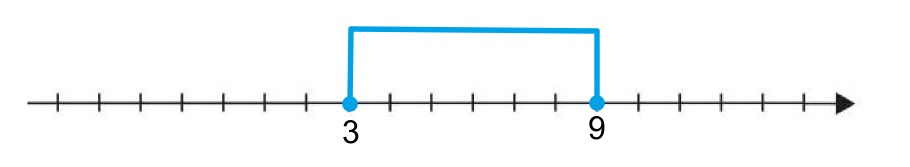
\includegraphics[scale=0.5]{warbez.jpeg}
		\end{figure}	
		Nierówność opisującą ten przedział można opisać za pomocą:
	}{$|x+6|\leq3$}{$|x-6|\leq3$}{$|x+6|\geq3$}{$|x-6|\geq3$}
	
	\ZadanieABCD{Dana jest liczba określona wzorem
	$$3\log_6\frac{1}{2}-\log_63+2\log_6\frac{1}{3}.$$ Liczba ta jest równa}{$2$}{$\frac{1}{2}$}{$-1$}{$-3$}

	\Zadanie{2}{\textbf{Wykaż, że wyrażenie $4n^2+6n+6$ dla każdej $n$ naturalnej jest liczbą parzystą.}}

	\ZadanieABCD{Wartość wyrażenia $(2a-3b)^2-(-2a-3b)^2$ wynosi}{$24ab$}{$18b^2$}{$-24ab$}{$0$}
	
	
	\ZadanieABCD{Dla pewnego ostrego kąta $\alpha$ dane jest, że $\sin\alpha = \frac{2\sqrt{2}}{3}$. Wówczas $\text{tg }\alpha$ wynosi}{$2\sqrt{2}$}{$\frac{\sqrt{2}}{4}$}{$3$}{$\frac{1}{3}$}
	
	\ZadanieABCD{Rówanie \large$\frac{(x^2-5)(x-3)}{(-2x+6)(x-5)}$$=0\quad$\normalsize ma }{zero rozwiązań}{jedno rozwiązanie}{dwa rozwiązania}{trzy rozwiązania}
	
	\Zadanie{3}{\textbf{Rozwiąż równanie}
		$$x^6-8=7x^3$$}
	
	\ZadanieABCDEF{	Poniżej podano pary pewnych prostych.
		\\
		
		Pary prostych prostopadłych to pary: ...... i ...... .}{$y=4x-5$ i $y=\frac{1}{4}x-5$}{$y=\frac{1}{4}x+5$ i $y=-4x+5$}{$y=4x-5$ i $y=4x-\sqrt{5}$}{$2x-3y-7=0$ i $2x+3y+7=0$}{$4x-5y+6=0$ i $5x+4y-6=0$}{$x+5y+4=0$ i $5x+y-4=0$}
	\newpage
	\
	\Informacja{3}
	W kartezjańskim układzie współrzędnych (x,y) przedstawiono fragment funkcji kwadratowej $f$ (zobacz rysunek). Jej wierzchołek to punkt $(5,8)$, natomiast jednym z jej miejsc zerowych jest $x=3$.
	
	\begin{figure}[h]
		\centering
		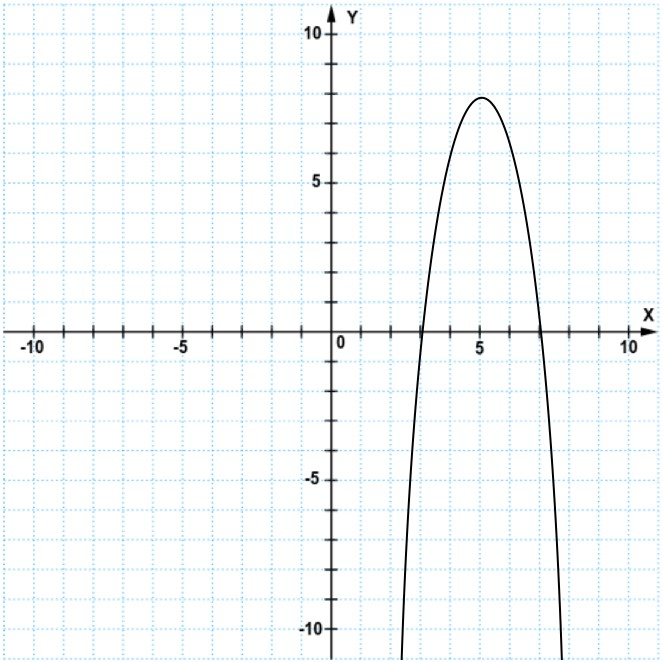
\includegraphics[scale=0.7]{pm1.jpeg}
	\end{figure}
	
	\SubZadanie{1}{Zapisz poniżej w postaci przedziału zbiór wartości powyższej funkcji kwadratowej. \vspace{1cm}
		
		....................................................................................................................................}
	
	
	
	\SubZadanie{2}{Wyznacz wzór funkcji kwadratowej w postaci ogólnej.}

			\begin{tabular}{|p{0.1cm}|p{0.1cm}|p{0.1cm}|p{0.1cm}|p{0.1cm}|p{0.1cm}|p{0.1cm}|p{0.1cm}|p{0.1cm}|p{0.1cm}|p{0.1cm}|p{0.1cm}|p{0.1cm}|p{0.1cm}|p{0.1cm}|p{0.1cm}|p{0.1cm}|p{0.1cm}|p{0.1cm}|p{0.1cm}|p{0.1cm}|p{0.1cm}|p{0.1cm}|p{0.1cm}|p{0.1cm}|p{0.1cm}|p{0.1cm}|p{0.1cm}|p{0.1cm}|p{0.1cm}|p{0.1cm}|p{0.1cm}}
		\hline&&&&&&&&&&&&&&&&&&&&&&&&&&&&&&\\
		\hline&&&&&&&&&&&&&&&&&&&&&&&&&&&&&&\\
		\hline&&&&&&&&&&&&&&&&&&&&&&&&&&&&&&\\
		\hline&&&&&&&&&&&&&&&&&&&&&&&&&&&&&&\\
		\hline&&&&&&&&&&&&&&&&&&&&&&&&&&&&&&\\
		\hline&&&&&&&&&&&&&&&&&&&&&&&&&&&&&&\\
		\hline&&&&&&&&&&&&&&&&&&&&&&&&&&&&&&\\
		\hline
	\end{tabular}

	\SubZadanie{1}{Funkcję $g(x)=f(x-2)-2$ przedstawiono na wykresie \begin{figure}[h]
			\centering
			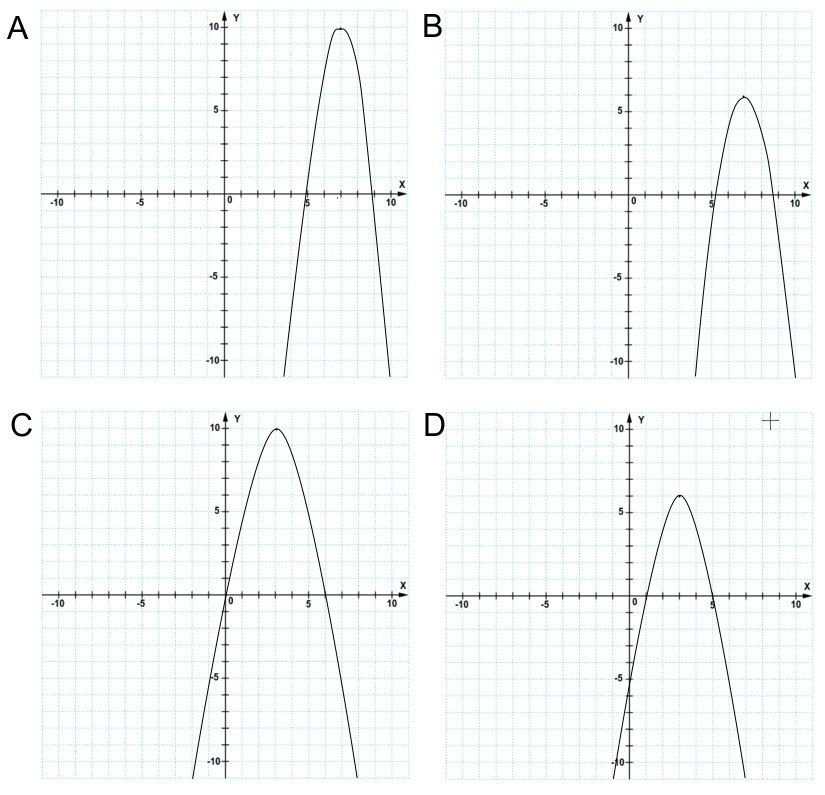
\includegraphics[scale=0.5]{pm2.jpeg}
	\end{figure}}
	
	
	

	\stepcounter{counter}

	\ZadanieABCD{W laboratorium badano próbki pewnego kamienia pozaziemskiego. Naukowcy są w stanie ustalić wiek powstania danego kamienia na postawie śladu węgla wewnątrz danej probówki za pomocą uproszczonej formuły $T(x)= 1000\cdot2^{-x \cdot 10^{-10}}$ w jednej uncji próbki (wyrażonej w mg), gdzie x to jest czas życia danej probówki.
		\\\\
		Przy badaniu tej próbki otrzymano, że w jednej uncji znajduje się 62,5mg węgla. Zatem ten kamień ma}{$4\cdot10^{10}$ lat}{$4000$ lat}{$62,5\cdot10^{10}$ lat}{$62,5\cdot 10^{10000} $ lat}
	
	\ZadaniePF{Dany jest ciąg rekurencyjny określony wzorem $$\left\{\begin{array}{l}
			a_{n+1}=a_n\cdot2n\\
			a_1=3
		\end{array}\right.$$}{Ciąg $a_n$ jest ciągiem geometrycznym.}{Ciąg $a_n$ jest ciągiem monotonicznym.}
	
	\ZadaniePF{Suma pierwszego i dwunastego wyrazu pewnego ciągu arytmetycznego wynosi 4, natomiast różnica piątego i siódmego wyrazu tego ciągu wynosi 4.}{Ciąg ten jest rosnący.}{Pierwszy wyraz tego ciągu wynosi 13.}
	
	\Zadanie{4}{Dany jest pewien trzywyrazowy ciąg arytmetyczny $(x,y,z)$. Średnia arytmetyczna tego ciągu to $7$. Jeżeli drugi wyraz tego ciągu zmniejszylibyśmy o $1$, a trzeci wyraz zwiększyli o 1, to otrzymalibyśmy ciąg geometryczny. Wyznacz wyrazy tego ciągu.}
	\\\\
				\begin{tabular}{|p{0.1cm}|p{0.1cm}|p{0.1cm}|p{0.1cm}|p{0.1cm}|p{0.1cm}|p{0.1cm}|p{0.1cm}|p{0.1cm}|p{0.1cm}|p{0.1cm}|p{0.1cm}|p{0.1cm}|p{0.1cm}|p{0.1cm}|p{0.1cm}|p{0.1cm}|p{0.1cm}|p{0.1cm}|p{0.1cm}|p{0.1cm}|p{0.1cm}|p{0.1cm}|p{0.1cm}|p{0.1cm}|p{0.1cm}|p{0.1cm}|p{0.1cm}|p{0.1cm}|p{0.1cm}|p{0.1cm}|p{0.1cm}}
		\hline&&&&&&&&&&&&&&&&&&&&&&&&&&&&&&\\
		\hline&&&&&&&&&&&&&&&&&&&&&&&&&&&&&&\\
		\hline
	\end{tabular}

	\ZadanieABCD{Dany jest trójkąt równoramienny o ramieniu długości 20 i kącie między ramionami $150^\circ$. Wówczas pole tego trójkąta jest równe}{$200\sqrt{3}$}{$200$}{$100\sqrt{3}$}{$100$}
	
	\ZadanieABCD{W trójkącie prostokątnym $ABC$ o kącie prostym przy wierzchołku $B$, kącie $30^\circ$ przy wierzchołku $A$ i boku $BC$ równym 4, poprowadzono prostą z wierzchołka $C$ przecinającą bok $AB$ w puncie $D$ pod kątem $45^\circ$. (Zobacz rysunek)
		
	\begin{figure}[h]
		\centering
		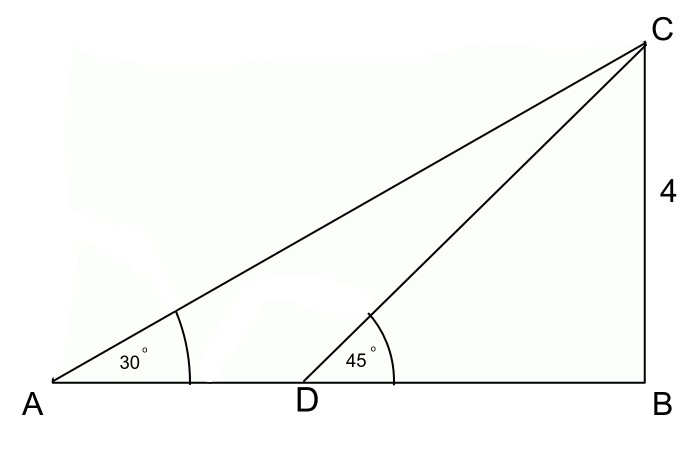
\includegraphics[scale=0.5]{pm3.jpeg}
	\end{figure}
	
	Długość odcinka $AD$ jest równa
	}{$8\sqrt{3}$}{$4(\sqrt{3}-1)$}{$4(\sqrt{2}+1)$}{$\sqrt{3}$}

	\Zadanie{3}{Dany jest trójkąt ostrokątny $ABC$ o kącie $ACB$, którego sinus wynosi $\frac{3\sqrt{11}}{10}$ oraz boki $AC$ i $BC$ są odpowiednio równe 5 i 8. Oblicz bok $AB$ tego trójkąta.}
	\\\\
	\begin{tabular}{|p{0.1cm}|p{0.1cm}|p{0.1cm}|p{0.1cm}|p{0.1cm}|p{0.1cm}|p{0.1cm}|p{0.1cm}|p{0.1cm}|p{0.1cm}|p{0.1cm}|p{0.1cm}|p{0.1cm}|p{0.1cm}|p{0.1cm}|p{0.1cm}|p{0.1cm}|p{0.1cm}|p{0.1cm}|p{0.1cm}|p{0.1cm}|p{0.1cm}|p{0.1cm}|p{0.1cm}|p{0.1cm}|p{0.1cm}|p{0.1cm}|p{0.1cm}|p{0.1cm}|p{0.1cm}|p{0.1cm}|p{0.1cm}}
		\hline&&&&&&&&&&&&&&&&&&&&&&&&&&&&&&\\
		\hline&&&&&&&&&&&&&&&&&&&&&&&&&&&&&&\\
		\hline&&&&&&&&&&&&&&&&&&&&&&&&&&&&&&\\
		\hline&&&&&&&&&&&&&&&&&&&&&&&&&&&&&&\\
		\hline&&&&&&&&&&&&&&&&&&&&&&&&&&&&&&\\
		\hline&&&&&&&&&&&&&&&&&&&&&&&&&&&&&&\\
		\hline&&&&&&&&&&&&&&&&&&&&&&&&&&&&&&\\
		\hline
	\end{tabular}

	\ZadanieABCD{Dany jest okrąg o środku w punkcie $(2,4)$ styczny do osi $OX$. Jednym z punktów przecięcia tego okręgu z osią $OY$ to
	}{$(0,4+2\sqrt{3})$}{$(0,2+\sqrt{3})$}{$(2+2\sqrt{3},0)$}{$(4+2\sqrt{3},0)$}
	
	\ZadanieABCD{Na okręgu o środku w punkcie $O$ zaznaczono punkty $A,B,C$ tak, że środkiem odcinka $BC$ jest punkt $O$. W punkcie $C$ poprowadzoną styczną do tego okręgu, która wraz z odcinkiem $AC$ tworzy kąt $70^\circ$. (Zobacz rysunek) 
		
		\begin{figure}[h]
			\centering
			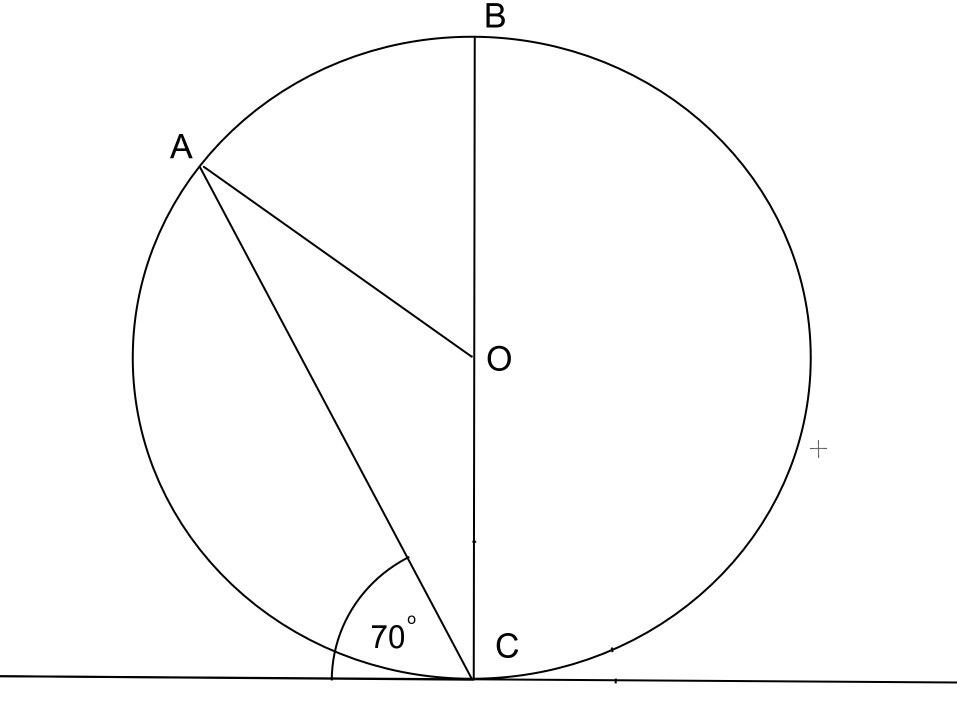
\includegraphics[scale=0.5]{pm4.jpeg}
		\end{figure}
		
		Miara kąta $\angle$ $AOB$ jest równa}{$70^\circ$}{$40^\circ$}{$35^\circ$}{$20^\circ$}
	
	
	\ZadanieABCD{Dane są dwa okręgi
		$$o_1\;:\;(x-2)^2+(y-k)^2=81$$
		$$o_2\;:\;(x+2)^2+(y-6)^2=16$$
		
		Okręgi te są styczne wewnętrznie kiedy $k$ jest równe}{$3-3\sqrt{15}$}{$3$}{$6$}{$-1$}

	\newpage

	\Zadanie{3}{W gniastosłupie prawidłowym czworokątnym wysokość graniastosłupa wynosi 8, a sinus kąta nachylenia przekątnej graniastosłupa do podstawy wynosi $\frac{\sqrt{6}}{3}$. Oblicz objętość tego graniastosłupa.}
	\\\\
	\begin{tabular}{|p{0.1cm}|p{0.1cm}|p{0.1cm}|p{0.1cm}|p{0.1cm}|p{0.1cm}|p{0.1cm}|p{0.1cm}|p{0.1cm}|p{0.1cm}|p{0.1cm}|p{0.1cm}|p{0.1cm}|p{0.1cm}|p{0.1cm}|p{0.1cm}|p{0.1cm}|p{0.1cm}|p{0.1cm}|p{0.1cm}|p{0.1cm}|p{0.1cm}|p{0.1cm}|p{0.1cm}|p{0.1cm}|p{0.1cm}|p{0.1cm}|p{0.1cm}|p{0.1cm}|p{0.1cm}|p{0.1cm}|p{0.1cm}}
		\hline&&&&&&&&&&&&&&&&&&&&&&&&&&&&&&\\
		\hline&&&&&&&&&&&&&&&&&&&&&&&&&&&&&&\\
		\hline&&&&&&&&&&&&&&&&&&&&&&&&&&&&&&\\
		\hline&&&&&&&&&&&&&&&&&&&&&&&&&&&&&&\\
		\hline&&&&&&&&&&&&&&&&&&&&&&&&&&&&&&\\
		\hline&&&&&&&&&&&&&&&&&&&&&&&&&&&&&&\\
		\hline&&&&&&&&&&&&&&&&&&&&&&&&&&&&&&\\
		\hline
	\end{tabular}

	\ZadanieABCD{Dany jest ostrosłup prawidłowy o boku podstawy równym 4 oraz kącie nachylenia wysokości ściany bocznej do podstawy, takim, że $\cos\alpha=\frac{4}{5}$. (Zobacz rysunek)
		
		\begin{figure}[h]
			\centering
			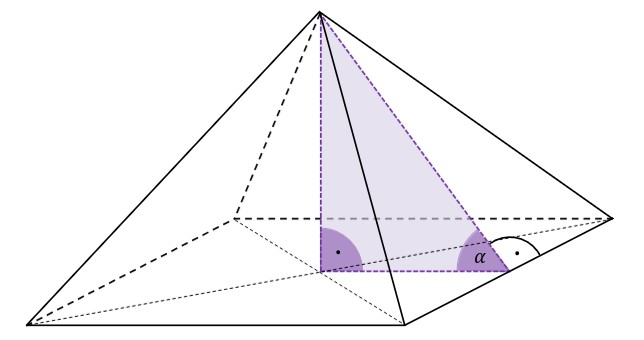
\includegraphics[scale=0.8]{pm5.jpeg}
		\end{figure}
		
		Objętość tego ostrosłupa jest równa}{$48$}{$16$}{$\frac{16\sqrt{17}}{3}$}{$8$}

	\ZadanieABCD{Liczb czterocyfrowych, w których występuje przynajmniej raz cyfra 5 jest
	}{$7700$}{$4000$}{$3439$}{$3168$}

	\Zadanie{2}{Dane są dwie urny, w pierwsze urnie są 4 kule białe i 6 czarnych, a w drugiej 3 białe i 5 czarnych. Doświadczenie polega na rzuceniu symetryczną monetą, a następnie jeśli wypadnie orzeł to losowaniu kuli z urny pierwszej, a jeśli wypadnie reszka to losowaniu kuli z urny drugiej. Oblicz prawdopodobieństwo wylosowania kuli białej.}
	
	\ZadanieABCD{Średnia arytmetyczna liczb: $x+3,\;5,\;7,\;3x,\;4,\;2x-3,\;3-x$ wynosi 2. Liczba $x$ wynosi}{$-1$}{$2$}{$2,5$}{$4$}

	\ZadanieABCD{Poniżej przedstawiono interpretację geometryczną układu równań.
		\begin{center}
			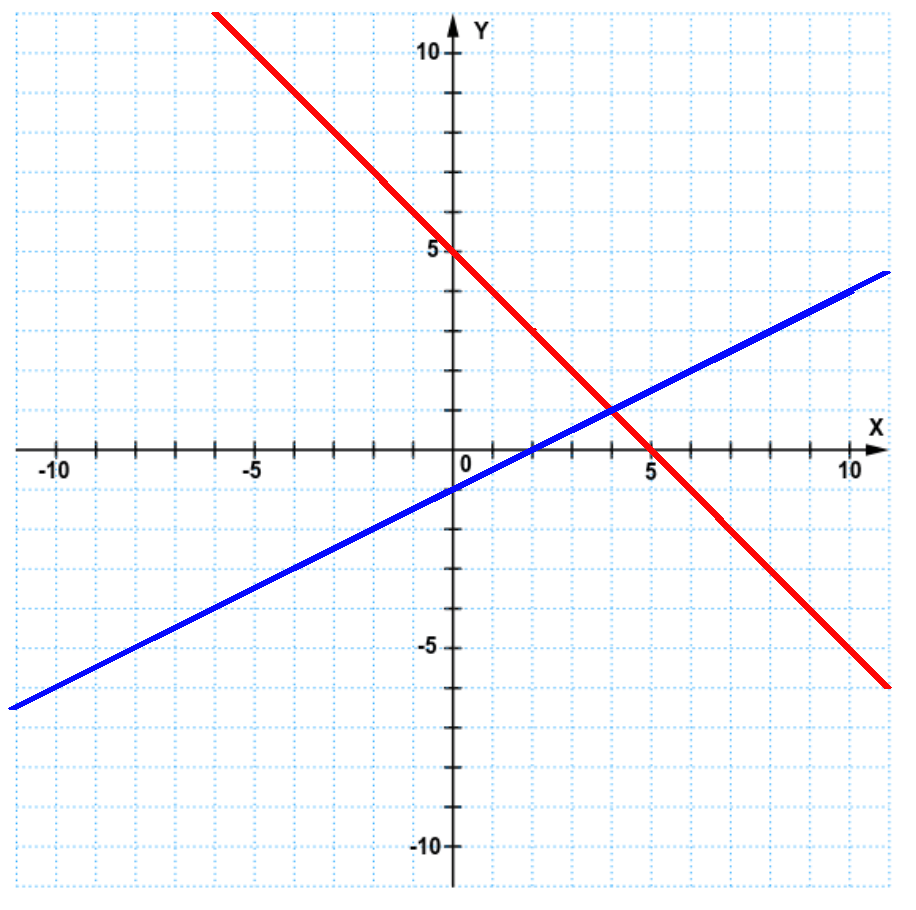
\includegraphics[scale=0.3]{lin_zd.png}
		\end{center}
		Układ ten da się zapisać w postaci}
	{\UkladRownan{y=x+5}{y=2x-1}}
	{\UkladRownan{y=-x-5}{y=2x+2}}
	{\UkladRownan{y=-x+5}{y=\frac{1}{2} x-1}}
	{\UkladRownan{y=x-5}{y=-\frac{1}{2} x+2}}
	
	\newpage
	
	\Zadanie{4}{
		Pan Andrzej na środku pola chce wytyczyć działkę w następujący sposób (zobacz rysunek):
		\begin{itemize}
			\item podzielić działkę na trzy prostokąty,
			\item dwa z nich mają mieć identyczne długości boków,
			\item każdą z tych części ogrodzić płotem, którego ma do dyspozycji 300 m (fragmenty działki współdzielące płot liczy się tylko raz).
		\end{itemize}
		\begin{figure}[h]
			\centering
			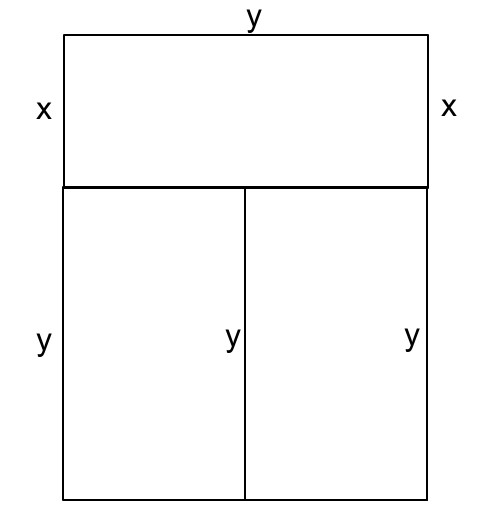
\includegraphics[scale=0.6]{optymal.jpeg}
		\end{figure}
		Wyznacz wymiary działki tak, aby jej pole powierzchni było jak największe. Oblicz to pole.
	}
	

\end{document}
